\section{Konzept}

    \subsection{Architektur}
    \begin{figure}[H]
        \centering
        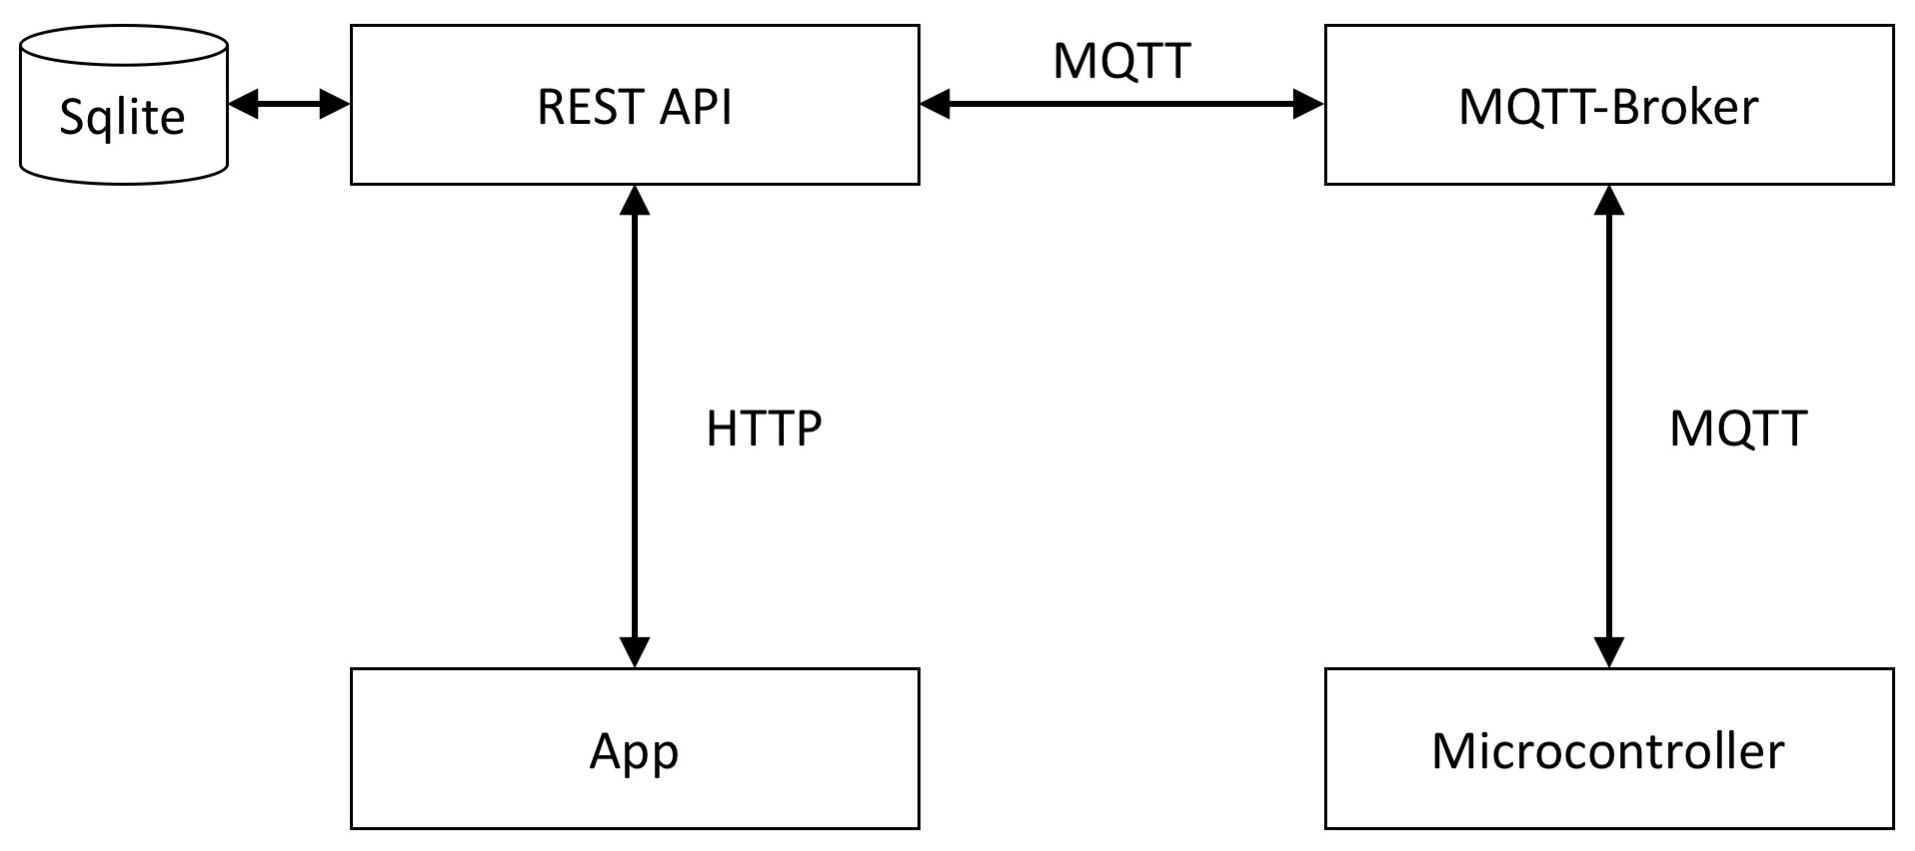
\includegraphics[width=0.7\linewidth]{../Pictures/Konzept/Architecture}
        \caption{Projektarchitektur}
        \label{fig:architecture}
    \end{figure}
    
    \subsection{Datenmodell}
    
    \subsection{Mobile Applikation}

        \subsubsection{React Native}
        \subsubsection{Views}

    \subsection{REST-API}

        \subsubsection{Django}
        \subsubsection{Ressourcen}
        \newcommand{\tabitem}{~~\llap{\textbullet}~~}
     \begin{minipage}{\textwidth}
             GET controller/\{controllerID\}/ 
        
          \begin{tabularx}{\textwidth}{lX}
                \toprule Beschreibung & Überprüft Validität der Controller-ID \\
                URL-Parameter & controllerID: zu überprüfende ID des Controllers \\
                Body & - \\
                Response & \{ "exists": true/false\}
            \end{tabularx}
    \end{minipage}\\\\
        
     \begin{minipage}{\textwidth}
            GET controller/\{controllerID\}/plant/ 

          \begin{tabularx}{\textwidth}{lX}
                \toprule Beschreibung & Alle Pflanzen des Microcontrollers \\
                URL-Parameter & controllerID: ID des Controllers mit dem die Pflanzen verbunden sind \\
                Body & - \\
                Response & Liste von Pflanzen
            \end{tabularx}
    \end{minipage}\\\\
        
     \begin{minipage}{\textwidth}
             POST  controller/\{controllerID\}/plant/ 
         
          \begin{tabularx}{\textwidth}{lX}
             \toprule Beschreibung & Erstellt eine neue Pflanze \\
             URL-Parameter & controllerID: ID des Controllers mit dem die Pflanzen verbunden sind \\
             Body & Zu erstellende Pflanze ohne ID \\
             Response & Erstellte Pflanze mit ID
         \end{tabularx}
    \end{minipage}\\\\
     
     \begin{minipage}{\textwidth}
              GET  controller/\{controllerID\}/plant/\{plantID\} 
          
          \begin{tabularx}{\textwidth}{lX}
              \toprule Beschreibung & Alle Informationen zu einer spezifischen Pflanze \\
              URL-Parameter & 
                  \begin{tabular}[t]{ll}
                       \tabitem controllerID: ID des Controllers mit dem die Pflanzen verbunden sind \\ 
                       \tabitem plantID: Eindeutige ID der angefragten Pflanze
                  \end{tabular}\\
              Body & - \\
              Response & Pflanzenobjekt
          \end{tabularx}
    \end{minipage}\\\\
          
     \begin{minipage}{\textwidth}
              PUT controller/\{controllerID\textgreater/plant/\{plantID\} 
          
            \begin{tabularx}{\textwidth}{lX}
              \toprule Beschreibung & Updated eine existierende Pflanze \\
              URL-Parameter & 
              \begin{tabular}[t]{ll}
                  \tabitem controllerID: ID des Controllers mit dem die Pflanzen verbunden sind \\ 
                  \tabitem plantID: Eindeutige ID der zu updatenden Pflanze
              \end{tabular}\\
              Body & Geändertes Pflanzenobjekt \\
              Response & Geändertes Pflanzenobjekt
          \end{tabularx}
    \end{minipage}\\\\
      
     \begin{minipage}{\textwidth}
         
              DELETE controller/\{controllerID\}/plant/\{plantID\}/ 
          
          \begin{tabularx}{\textwidth}{lX}
              \toprule Beschreibung & Löschen einer Pflanze \\
              URL-Parameter & 
              \begin{tabular}[t]{ll}
                  \tabitem controllerID: ID des Controllers mit dem die Pflanzen verbunden sind \\ 
                  \tabitem plantID: Eindeutige ID der zu löschenden Pflanze
              \end{tabular}\\
              Body & - \\
              Response & -
          \end{tabularx}
        \end{minipage}\\\\
      
     \begin{minipage}{\textwidth}
         
              GET  controller/\{controllerID\}/plant/\{plantID\}/moisture 
          
          \begin{tabularx}{\textwidth}{lX}
              \toprule Beschreibung & Abfragen aller Feuchtigkeitsmessungen für eine Pflanze \\
              URL-Parameter & 
              \begin{tabular}[t]{ll}
                  \tabitem controllerID: ID des Controllers mit dem die Pflanzen verbunden sind \\ 
                  \tabitem plantID: Eindeutige ID der Pflanze
              \end{tabular}\\
              Body & - \\
              Response & Liste an Feuchtigkeitswerten
          \end{tabularx}
        \end{minipage}\\
      
     \begin{minipage}{\textwidth}
             
      POST controller/\{controllerID\}/plant/\{plantID\}/water/\{amount\} 
      
          \begin{tabularx}{\textwidth}{lX}
          \toprule Beschreibung & Bewässerung einer Pflanze \\
          URL-Parameter & 
          \begin{tabular}[t]{ll}
              \tabitem controllerID: ID des Controllers mit dem die Pflanzen verbunden sind \\ 
              \tabitem plantID: Eindeutige ID der zu bewässernden Pflanze \\
              \tabitem amount: Wassermenge in Millilitern
          \end{tabular}\\
          Body & - \\
          Response & -
      \end{tabularx}
  \end{minipage}\\

    \subsection{Microcontroller}


        \subsubsection{Kommunikation}
        Zur Kommunikation wird das Protokoll \textit{MQTT} verwendet. MQTT ist ein leichtgewichtiges Nachrichtenprotokoll, welches auf TCP/ IP aufbaut. Es ist wurde speziell für Anwendungen mit geringen Ressourcen sowie für limitierten Bandbreite entworfen. Damit eignet es sich sehr gut für Internet-of-Things-Anwendungen, wird aber auch zunehmend bei mobilen Applikationen genutzt.
        
        MQTT setzt das Publish-Subscribe-Pattern um. Server und Microcontroller sind beide Clients, die sich mit einem gemeinsamen MQTT-Broker verbinden. Dort können sie sich für Benachrichtigungen zu speziellen Themen anmelden (subscribe). Themen werden als URL dargestellt. Inhalte zu einem Thema können veröffentlicht (publish) werden. Der Broker benachrichtigt dann automatisch alle Clients, welche sich für das Thema eingeschrieben haben.\\
        
        Die Form der gesendeten Daten unterscheidet sich teilweise etwas vom gewohnten Vorgehen mit leistungsstärkeren Geräten. Die Form ist darauf ausgelegt zu jeder Zeit eine minimale Menge an Daten auf dem Microcontroller vorzuhalten sowie diese möglichst leichtgewichtig lesbar zu machen.\\
        
        \begin{minipage}{\textwidth}
            WateringOfPlants/microController/\{controllerID\}/water
            
            \begin{tabularx}{\textwidth}{lX}
                \toprule Beschreibung & Anweisung vom Server eine Pflanze zu bewässern  \\
                URL-Parameter & controllerID: ID des Controllers der die Pflanze bewässern soll\\
                Daten & 
                  \begin{tabular}[t]{ll}
                      \{ \\
                          \tab "position": <position>, \\
                          \tab "time": <time> \\
                      \} \\
                    \tabitem position: Position der Pflanze in Grad \\ 
                    \tabitem time: Zeit in Millisekunden für die die Pumpe aktiviert werden soll
                \end{tabular}\\
            \end{tabularx}
        \end{minipage}\\
    
        WateringOfPlants/microController/\{controllerID\}/measure
        
        \begin{minipage}{\textwidth}
            \begin{tabularx}{\textwidth}{lX}
                \toprule Beschreibung & Anweisung vom Server die Feuchtigkeitswerte zu erheben  \\
                URL-Parameter & controllerID: ID des Controllers der die Werte erheben soll\\
                Daten & 
                \begin{tabular}[t]{ll}
                    \{ \\
                    \tab "pins": [<pinNr>, <pinNr> ... ]>, \\
                    \tab "nrOfPins": <nrOfPins> \\
                    \} \\
                    \tabitem pins: Pins an denen die Feuchtigkeitssensoren angeschlossen sind \\ 
                    \tabitem nrOfPins: Länge des pins-Arrays
                \end{tabular}\\
            \end{tabularx}
        \end{minipage}\\
    
    
        WateringOfPlants/microController/\{controllerID\}/measuredValues/\{pinNr\}
        
        \begin{minipage}{\textwidth}
            \begin{tabularx}{\textwidth}{lX}
                \toprule Beschreibung & Gemessener Feuchtigkeitswert vom Microcontroller  \\
                URL-Parameter &  
                \begin{tabular}[t]{ll}
                    \tabitem controllerID: ID des Controllers, der den Feuchtigkeitswert erhoben hat.\\ 
                    \tabitem pinNr: Pin zu welchem der Feuchtigkeitswert erhoben wurde
                \end{tabular}\\
                Daten & 
                \begin{tabular}[t]{ll}
                    <moistureValue> \\
                    \tabitem moistureValue: Erhobener Feuchtigkeitswert als Double
                \end{tabular}\\
            \end{tabularx}
        \end{minipage}\\
    
        \subsubsection{Verwendete Hardwarekomponenten}

    \subsection{Codequalität}